\documentclass[10pt,a4paper,draft]{article}
\usepackage[utf8x]{inputenc}
\usepackage{ucs}
\usepackage[english]{babel}
\usepackage{multirow}
\usepackage{rotating}
\author{Lukáš Petrovický}
\title{RAS2012: Competition Entry}
\begin{document}

\maketitle

\begin{abstract}
This article describes an entry to the 2012 RAS Problem Solving Competition, concerning dispatching on multi-track territories. The entry is based on the Drools Planner, a Java-based solver. On a reasonably recent computer, the resulting algorithm is able to produce feasible results within a minute and has been fine-tuned to provide best results in under 3 minutes. Source code to the entry is open source and well documented.
\end{abstract}

\section{Introduction}

\section{Describing the solution}

\section{Implementation}

\section{Conclusion}

\appendix

\section{Resolved systems}

In this section, we show the best solutions reached for each data set. All these were reached within 3 minutes in a single-threaded run, using Intel i7 Q820 processor running Fedora 17 and 1 GB of heap space inside Java 7 runtime environment. The specific solver configurations used to reach these solutions may not have been the same every time.

Please note that via the benchmarking functionality of Drools planner (see above), users may be able to fine-tune the algorithm. This fine-tuning can be focused either on providing better solutions or on faster turnaround times.

\begin{sidewaystable}
\footnotesize
\caption{Statistics for resolved system ``RAS DATA SET 1'', costing \$1280.}
\centering
\begin{tabular}{c||c|c||c|c|c|c|c||c|c|c}
  \hline \hline
  &
  Unpref. & 
  Delay &
  Node &
  When &
  SA &
  +/- &
  Pty &
  TWT &
  +/- &
  Pty \\
      \hline
      \multirow{2}{*}{A1} &
      \multirow{2}{*}{0} &
      \multirow{2}{*}{0} &
      37 &
      2398.5 &
      3600 &
        1201.5 &
        0 &
      \multirow{2}{*}{5400} &
        \multirow{2}{*}{67.5} &
        \multirow{2}{*}{0}
      \\
      \cline{4-8}
       &
       &
       &
      39 &
      5332.5 &
      7800 &
        2467.5 &
        0 &
      
         &
        
      \\
      \hline
      \multirow{2}{*}{A2} &
      \multirow{2}{*}{4} &
      \multirow{2}{*}{0} &
      37 &
      6124.742 &
      7800 &
        1675.258 &
        0 &
      \multirow{2}{*}{9000} &
        \multirow{2}{*}{82.412} &
        \multirow{2}{*}{0}
      \\
      \cline{4-8}
       &
       &
       &
      39 &
      8917.588 &
      12000 &
        3082.412 &
        0 &
      
         &
        
      \\
      \hline
      \multirow{2}{*}{B1} &
      \multirow{2}{*}{18} &
      \multirow{2}{*}{2700} &
      37 &
      12210.388 &
      12600 &
        389.612 &
        0 &
      \multirow{2}{*}{13800} &
        \multirow{2}{*}{-4171.478} &
        \multirow{2}{*}{0}
      \\
      \cline{4-8}
       &
       &
       &
      0 &
      17971.478 &
      17400 &
        -571.478 &
        0 &
      
         &
        
      \\
      \hline
      \multirow{2}{*}{B2} &
      \multirow{2}{*}{0} &
      \multirow{2}{*}{0} &
      37 &
      13621.758 &
      15600 &
        1978.242 &
        0 &
      \multirow{2}{*}{16800} &
        \multirow{2}{*}{-538.224} &
        \multirow{2}{*}{0}
      \\
      \cline{4-8}
       &
       &
       &
      39 &
      17338.224 &
      19800 &
        2461.776 &
        0 &
      
         &
        
      \\
      \hline
      \multirow{2}{*}{B3} &
      \multirow{2}{*}{6} &
      \multirow{2}{*}{2160} &
      37 &
      41166.616 &
      40200 &
        -966.616 &
        0 &
      \multirow{2}{*}{42000} &
        \multicolumn{2}{c}{\multirow{2}{*}{N/A}}
      \\
      \cline{4-8}
       &
       &
       &
      39 &
      44133.756 &
      45000 &
        \multicolumn{2}{|c||}{N/A} &
      
        
      \\
      \hline
      \multirow{2}{*}{C1} &
      \multirow{2}{*}{0} &
      \multirow{2}{*}{0} &
      37 &
      17598 &
      19200 &
        1602 &
        0 &
      \multirow{2}{*}{21600} &
        \multirow{2}{*}{282} &
        \multirow{2}{*}{0}
      \\
      \cline{4-8}
       &
       &
       &
      39 &
      21318 &
      24600 &
        3282 &
        0 &
      
         &
        
      \\
      \hline
      \multirow{2}{*}{C2} &
      \multirow{2}{*}{0} &
      \multirow{2}{*}{0} &
      37 &
      25700.145 &
      27000 &
        1299.855 &
        0 &
      \multirow{2}{*}{28800} &
        \multirow{2}{*}{-1181.575} &
        \multirow{2}{*}{0}
      \\
      \cline{4-8}
       &
       &
       &
      39 &
      29981.575 &
      33000 &
        3018.425 &
        0 &
      
         &
        
      \\
      \hline
      \multirow{2}{*}{D1} &
      \multirow{2}{*}{0} &
      \multirow{2}{*}{0} &
      37 &
      26334.852 &
      29400 &
        3065.148 &
        0 &
      \multirow{2}{*}{31200} &
        \multirow{2}{*}{296.584} &
        \multirow{2}{*}{0}
      \\
      \cline{4-8}
       &
       &
       &
      0 &
      30903.416 &
      36600 &
        5696.584 &
        0 &
      
         &
        
      \\
      \hline
      \multirow{2}{*}{D2} &
      \multirow{2}{*}{12} &
      \multirow{2}{*}{2160} &
      37 &
      21020.177 &
      21600 &
        579.823 &
        0 &
      \multirow{2}{*}{23400} &
        \multirow{2}{*}{-2105.604} &
        \multirow{2}{*}{0}
      \\
      \cline{4-8}
       &
       &
       &
      0 &
      25505.604 &
      28200 &
        2694.396 &
        0 &
      
         &
        
      \\
      \hline
      \multirow{2}{*}{D3} &
      \multirow{2}{*}{0} &
      \multirow{2}{*}{0} &
      37 &
      32868.738 &
      35400 &
        2531.262 &
        0 &
      \multirow{2}{*}{37200} &
        \multirow{2}{*}{102.361} &
        \multirow{2}{*}{0}
      \\
      \cline{4-8}
       &
       &
       &
      0 &
      37097.639 &
      41400 &
        4302.361 &
        0 &
      
         &
        
      \\
      \hline
      \multirow{2}{*}{E1} &
      \multirow{2}{*}{0} &
      \multirow{2}{*}{9240} &
      37 &
      43107 &
      36000 &
        -7107 &
        0 &
      \multirow{2}{*}{39000} &
        \multicolumn{2}{c}{\multirow{2}{*}{N/A}}
      \\
      \cline{4-8}
       &
       &
       &
      39 &
      48579 &
      44400 &
        \multicolumn{2}{|c||}{N/A} &
      
        
      \\
      \hline
      \multirow{2}{*}{F1} &
      \multirow{2}{*}{0} &
      \multirow{2}{*}{0} &
      37 &
      50955.427 &
      57600 &
        \multicolumn{2}{|c||}{N/A} &
      \multirow{2}{*}{63000} &
        \multicolumn{2}{c}{\multirow{2}{*}{N/A}}
      \\
      \cline{4-8}
       &
       &
       &
      0 &
      61919.996 &
      75000 &
        \multicolumn{2}{|c||}{N/A} &
      
        
      \\
\end{tabular}
\label{table:RDS1.txt-1280.tex} 
\end{sidewaystable}.

\begin{sidewaystable}
\footnotesize
\caption{Statistics for resolved system ``RAS DATA SET 2'', costing \$7867.}
\centering
\begin{tabular}{c||c|c||c|c|c|c|c||c|c|c}
  \hline \hline
  &
  Unpref. & 
  Delay &
  Node &
  When &
  SA &
  +/- &
  Pty &
  TWT &
  +/- &
  Pty \\
      \hline
      \multirow{2}{*}{A1} &
      \multirow{2}{*}{13} &
      \multirow{2}{*}{0} &
      37 &
      2785.5 &
      3600 &
        814.5 &
        0 &
      \multirow{2}{*}{5400} &
        \multirow{2}{*}{94.5} &
        \multirow{2}{*}{0}
      \\
      \cline{4-8}
       &
       &
       &
      39 &
      5305.5 &
      7800 &
        2494.5 &
        0 &
      
         &
        
      \\
      \hline
      \multirow{2}{*}{A2} &
      \multirow{2}{*}{0} &
      \multirow{2}{*}{240} &
      37 &
      10897.265 &
      11400 &
        502.735 &
        0 &
      \multirow{2}{*}{12600} &
        \multirow{2}{*}{-1856.215} &
        \multirow{2}{*}{0}
      \\
      \cline{4-8}
       &
       &
       &
      39 &
      14456.215 &
      15600 &
        1143.785 &
        0 &
      
         &
        
      \\
      \hline
      \multirow{2}{*}{A3} &
      \multirow{2}{*}{12} &
      \multirow{2}{*}{0} &
      37 &
      17482.5 &
      18000 &
        517.5 &
        0 &
      \multirow{2}{*}{19800} &
        \multirow{2}{*}{-1120.5} &
        \multirow{2}{*}{0}
      \\
      \cline{4-8}
       &
       &
       &
      39 &
      20920.5 &
      22200 &
        1279.5 &
        0 &
      
         &
        
      \\
      \hline
      \multirow{2}{*}{A4} &
      \multirow{2}{*}{0} &
      \multirow{2}{*}{9420} &
      37 &
      45344.214 &
      31800 &
        \multicolumn{2}{|c||}{N/A} &
      \multirow{2}{*}{39000} &
        \multicolumn{2}{c}{\multirow{2}{*}{N/A}}
      \\
      \cline{4-8}
       &
       &
       &
      0 &
      48866.128 &
      36600 &
        \multicolumn{2}{|c||}{N/A} &
      
        
      \\
      \hline
      \multirow{2}{*}{B1} &
      \multirow{2}{*}{4} &
      \multirow{2}{*}{120} &
      37 &
      6848.112 &
      4800 &
        -2048.112 &
        0 &
      \multirow{2}{*}{9600} &
        \multirow{2}{*}{-770.46} &
        \multirow{2}{*}{0}
      \\
      \cline{4-8}
       &
       &
       &
      39 &
      10370.46 &
      9000 &
        -1370.46 &
        0 &
      
         &
        
      \\
      \hline
      \multirow{2}{*}{B2} &
      \multirow{2}{*}{0} &
      \multirow{2}{*}{0} &
      37 &
      31798.125 &
      26400 &
        -5398.125 &
        0 &
      \multirow{2}{*}{35400} &
        \multirow{2}{*}{78.375} &
        \multirow{2}{*}{0}
      \\
      \cline{4-8}
       &
       &
       &
      39 &
      35321.625 &
      31200 &
        -4121.625 &
        0 &
      
         &
        
      \\
      \hline
      \multirow{2}{*}{B3} &
      \multirow{2}{*}{12} &
      \multirow{2}{*}{3000} &
      37 &
      10207.716 &
      11400 &
        1192.284 &
        0 &
      \multirow{2}{*}{10800} &
        \multirow{2}{*}{-2834.147} &
        \multirow{2}{*}{0}
      \\
      \cline{4-8}
       &
       &
       &
      0 &
      13634.147 &
      16800 &
        3165.853 &
        0 &
      
         &
        
      \\
      \hline
      \multirow{2}{*}{C1} &
      \multirow{2}{*}{11} &
      \multirow{2}{*}{0} &
      37 &
      35829.006 &
      26400 &
        -9429.006 &
        123 &
      \multirow{2}{*}{39000} &
        \multirow{2}{*}{-148.856} &
        \multirow{2}{*}{0}
      \\
      \cline{4-8}
       &
       &
       &
      39 &
      39148.856 &
      31800 &
        -7348.856 &
        8 &
      
         &
        
      \\
      \hline
      \multirow{2}{*}{C2} &
      \multirow{2}{*}{0} &
      \multirow{2}{*}{0} &
      37 &
      198 &
      0 &
        -198 &
        0 &
      \multirow{2}{*}{3600} &
        \multirow{2}{*}{-318} &
        \multirow{2}{*}{0}
      \\
      \cline{4-8}
       &
       &
       &
      39 &
      3918 &
      5400 &
        1482 &
        0 &
      
         &
        
      \\
      \hline
      \multirow{2}{*}{C3} &
      \multirow{2}{*}{4} &
      \multirow{2}{*}{22260} &
      37 &
      43807.716 &
      20400 &
        \multicolumn{2}{|c||}{N/A} &
      \multirow{2}{*}{25200} &
        \multicolumn{2}{c}{\multirow{2}{*}{N/A}}
      \\
      \cline{4-8}
       &
       &
       &
      0 &
      47541.004 &
      25800 &
        \multicolumn{2}{|c||}{N/A} &
      
        
      \\
      \hline
      \multirow{2}{*}{D1} &
      \multirow{2}{*}{0} &
      \multirow{2}{*}{0} &
      37 &
      40615.5 &
      43800 &
        3184.5 &
        0 &
      \multirow{2}{*}{44400} &
        \multicolumn{2}{c}{\multirow{2}{*}{N/A}}
      \\
      \cline{4-8}
       &
       &
       &
      39 &
      45430.5 &
      51000 &
        \multicolumn{2}{|c||}{N/A} &
      
        
      \\
      \hline
      \multirow{2}{*}{D2} &
      \multirow{2}{*}{0} &
      \multirow{2}{*}{0} &
      37 &
      2179.383 &
      3600 &
        1420.617 &
        0 &
      \multirow{2}{*}{6600} &
        \multirow{2}{*}{216.93} &
        \multirow{2}{*}{0}
      \\
      \cline{4-8}
       &
       &
       &
      39 &
      6383.07 &
      9600 &
        3216.93 &
        0 &
      
         &
        
      \\
      \hline
      \multirow{2}{*}{E1} &
      \multirow{2}{*}{31} &
      \multirow{2}{*}{2520} &
      37 &
      5552.184 &
      6600 &
        1047.816 &
        0 &
      \multirow{2}{*}{9600} &
        \multirow{2}{*}{-2190.003} &
        \multirow{2}{*}{0}
      \\
      \cline{4-8}
       &
       &
       &
      39 &
      11790.003 &
      14400 &
        2609.997 &
        0 &
      
         &
        
      \\
      \hline
      \multirow{2}{*}{E2} &
      \multirow{2}{*}{0} &
      \multirow{2}{*}{4680} &
      37 &
      5814.858 &
      1800 &
        -4014.858 &
        0 &
      \multirow{2}{*}{7200} &
        \multirow{2}{*}{-4706.294} &
        \multirow{2}{*}{0}
      \\
      \cline{4-8}
       &
       &
       &
      0 &
      11906.294 &
      10800 &
        -1106.294 &
        0 &
      
         &
        
      \\
      \hline
      \multirow{2}{*}{E3} &
      \multirow{2}{*}{0} &
      \multirow{2}{*}{43320} &
      37 &
      48987.427 &
      9000 &
        \multicolumn{2}{|c||}{N/A} &
      \multirow{2}{*}{12000} &
        \multicolumn{2}{c}{\multirow{2}{*}{N/A}}
      \\
      \cline{4-8}
       &
       &
       &
      0 &
      54469.71 &
      18000 &
        \multicolumn{2}{|c||}{N/A} &
      
        
      \\
      \hline
      \multirow{2}{*}{E4} &
      \multirow{2}{*}{18} &
      \multirow{2}{*}{0} &
      37 &
      27075.742 &
      30000 &
        2924.258 &
        0 &
      \multirow{2}{*}{32400} &
        \multirow{2}{*}{-91.404} &
        \multirow{2}{*}{0}
      \\
      \cline{4-8}
       &
       &
       &
      0 &
      32491.404 &
      37800 &
        5308.596 &
        0 &
      
         &
        
      \\
      \hline
      \multirow{2}{*}{F1} &
      \multirow{2}{*}{16} &
      \multirow{2}{*}{600} &
      37 &
      25388.18 &
      29400 &
        4011.82 &
        0 &
      \multirow{2}{*}{33600} &
        \multirow{2}{*}{179.456} &
        \multirow{2}{*}{0}
      \\
      \cline{4-8}
       &
       &
       &
      39 &
      33420.544 &
      41400 &
        7979.456 &
        0 &
      
         &
        
      \\
      \hline
      \multirow{2}{*}{F2} &
      \multirow{2}{*}{0} &
      \multirow{2}{*}{35280} &
      37 &
      56136.001 &
      30000 &
        \multicolumn{2}{|c||}{N/A} &
      \multirow{2}{*}{36000} &
        \multicolumn{2}{c}{\multirow{2}{*}{N/A}}
      \\
      \cline{4-8}
       &
       &
       &
      0 &
      69498.002 &
      51000 &
        \multicolumn{2}{|c||}{N/A} &
      
        
      \\
\end{tabular}
\label{table:RDS2.txt-7867.tex} 
\end{sidewaystable}.

\begin{sidewaystable}
\footnotesize
\caption{Statistics for resolved system ``RAS DATA SET 3'', costing \$12873.}
\centering
\begin{tabular}{c||c|c||c|c|c|c|c||c|c|c}
  \hline \hline
  &
  Unpref. & 
  Delay &
  Node &
  When &
  SA &
  +/- &
  Pty &
  TWT &
  +/- &
  Pty \\
      \hline
      \multirow{2}{*}{A1} &
      \multirow{2}{*}{0} &
      \multirow{2}{*}{0} &
      37 &
      1354.5 &
      2400 &
        1045.5 &
        0 &
      \multirow{2}{*}{4200} &
        \multirow{2}{*}{298.5} &
        \multirow{2}{*}{0}
      \\
      \cline{4-8}
       &
       &
       &
      39 &
      3901.5 &
      6000 &
        2098.5 &
        0 &
      
         &
        
      \\
      \hline
      \multirow{2}{*}{A2} &
      \multirow{2}{*}{13} &
      \multirow{2}{*}{3180} &
      37 &
      4500 &
      2400 &
        -2100 &
        0 &
      \multirow{2}{*}{4200} &
        \multirow{2}{*}{-3441.433} &
        \multirow{2}{*}{0}
      \\
      \cline{4-8}
       &
       &
       &
      0 &
      7641.433 &
      6600 &
        -1041.433 &
        0 &
      
         &
        
      \\
      \hline
      \multirow{2}{*}{A3} &
      \multirow{2}{*}{12} &
      \multirow{2}{*}{0} &
      37 &
      21754.288 &
      22800 &
        1045.712 &
        0 &
      \multirow{2}{*}{24000} &
        \multirow{2}{*}{-865.721} &
        \multirow{2}{*}{0}
      \\
      \cline{4-8}
       &
       &
       &
      0 &
      24865.721 &
      27000 &
        2134.279 &
        0 &
      
         &
        
      \\
      \hline
      \multirow{2}{*}{A4} &
      \multirow{2}{*}{0} &
      \multirow{2}{*}{9240} &
      37 &
      45104.214 &
      33600 &
        \multicolumn{2}{|c||}{N/A} &
      \multirow{2}{*}{39000} &
        \multicolumn{2}{c}{\multirow{2}{*}{N/A}}
      \\
      \cline{4-8}
       &
       &
       &
      0 &
      48412.881 &
      38400 &
        \multicolumn{2}{|c||}{N/A} &
      
        
      \\
      \hline
      \multirow{2}{*}{A5} &
      \multirow{2}{*}{12} &
      \multirow{2}{*}{4815} &
      37 &
      37084.5 &
      32400 &
        -4684.5 &
        0 &
      \multirow{2}{*}{34200} &
        \multirow{2}{*}{-5548.5} &
        \multirow{2}{*}{0}
      \\
      \cline{4-8}
       &
       &
       &
      39 &
      39748.5 &
      36600 &
        -3148.5 &
        0 &
      
         &
        
      \\
      \hline
      \multirow{1}{*}{B1} &
      \multirow{1}{*}{0} &
      \multirow{1}{*}{2400} &
      0 &
      4238.337 &
      1800 &
        -2438.337 &
        0 &
      \multirow{1}{*}{1200} &
        \multirow{1}{*}{-3038.337} &
        \multirow{1}{*}{0}
      \\
      \hline
      \multirow{1}{*}{B2} &
      \multirow{1}{*}{6} &
      \multirow{1}{*}{0} &
      39 &
      2951.799 &
      4800 &
        1848.201 &
        0 &
      \multirow{1}{*}{3000} &
        \multirow{1}{*}{48.201} &
        \multirow{1}{*}{0}
      \\
      \hline
      \multirow{2}{*}{B3} &
      \multirow{2}{*}{6} &
      \multirow{2}{*}{0} &
      37 &
      2977.488 &
      -3000 &
        -5977.488 &
        0 &
      \multirow{2}{*}{6000} &
        \multirow{2}{*}{-286.252} &
        \multirow{2}{*}{0}
      \\
      \cline{4-8}
       &
       &
       &
      39 &
      6286.252 &
      1800 &
        -4486.252 &
        0 &
      
         &
        
      \\
      \hline
      \multirow{2}{*}{B4} &
      \multirow{2}{*}{0} &
      \multirow{2}{*}{17700} &
      37 &
      46469.145 &
      16800 &
        \multicolumn{2}{|c||}{N/A} &
      \multirow{2}{*}{32400} &
        \multicolumn{2}{c}{\multirow{2}{*}{N/A}}
      \\
      \cline{4-8}
       &
       &
       &
      0 &
      49895.576 &
      21600 &
        \multicolumn{2}{|c||}{N/A} &
      
        
      \\
      \hline
      \multirow{1}{*}{C1} &
      \multirow{1}{*}{0} &
      \multirow{1}{*}{5880} &
      0 &
      9458.568 &
      6000 &
        -3458.568 &
        0 &
      \multirow{1}{*}{4200} &
        \multirow{1}{*}{-5258.568} &
        \multirow{1}{*}{0}
      \\
      \hline
      \multirow{2}{*}{C2} &
      \multirow{2}{*}{8} &
      \multirow{2}{*}{300} &
      37 &
      4003.288 &
      0 &
        -4003.288 &
        0 &
      \multirow{2}{*}{7200} &
        \multirow{2}{*}{-874.718} &
        \multirow{2}{*}{0}
      \\
      \cline{4-8}
       &
       &
       &
      39 &
      8074.718 &
      6000 &
        -2074.718 &
        0 &
      
         &
        
      \\
      \hline
      \multirow{2}{*}{C3} &
      \multirow{2}{*}{9} &
      \multirow{2}{*}{14940} &
      37 &
      47908.656 &
      30000 &
        \multicolumn{2}{|c||}{N/A} &
      \multirow{2}{*}{37200} &
        \multicolumn{2}{c}{\multirow{2}{*}{N/A}}
      \\
      \cline{4-8}
       &
       &
       &
      0 &
      52137.557 &
      36000 &
        \multicolumn{2}{|c||}{N/A} &
      
        
      \\
      \hline
      \multirow{2}{*}{D1} &
      \multirow{2}{*}{0} &
      \multirow{2}{*}{9120} &
      37 &
      13073.996 &
      4200 &
        -8873.996 &
        92 &
      \multirow{2}{*}{7800} &
        \multirow{2}{*}{-9537.683} &
        \multirow{2}{*}{0}
      \\
      \cline{4-8}
       &
       &
       &
      39 &
      17337.683 &
      10200 &
        -7137.683 &
        0 &
      
         &
        
      \\
      \hline
      \multirow{2}{*}{D2} &
      \multirow{2}{*}{10} &
      \multirow{2}{*}{1200} &
      37 &
      41411.998 &
      42000 &
        588.002 &
        0 &
      \multirow{2}{*}{43800} &
        \multicolumn{2}{c}{\multirow{2}{*}{N/A}}
      \\
      \cline{4-8}
       &
       &
       &
      39 &
      45610.147 &
      48000 &
        \multicolumn{2}{|c||}{N/A} &
      
        
      \\
      \hline
      \multirow{2}{*}{E1} &
      \multirow{2}{*}{0} &
      \multirow{2}{*}{42360} &
      37 &
      48891.433 &
      10200 &
        \multicolumn{2}{|c||}{N/A} &
      \multirow{2}{*}{13200} &
        \multicolumn{2}{c}{\multirow{2}{*}{N/A}}
      \\
      \cline{4-8}
       &
       &
       &
      0 &
      55546.581 &
      19200 &
        \multicolumn{2}{|c||}{N/A} &
      
        
      \\
      \hline
      \multirow{2}{*}{E2} &
      \multirow{2}{*}{45} &
      \multirow{2}{*}{4914} &
      37 &
      15777 &
      18000 &
        2223 &
        0 &
      \multirow{2}{*}{21000} &
        \multirow{2}{*}{-5019} &
        \multirow{2}{*}{0}
      \\
      \cline{4-8}
       &
       &
       &
      39 &
      26019 &
      26400 &
        381 &
        0 &
      
         &
        
      \\
      \hline
      \multirow{2}{*}{E3} &
      \multirow{2}{*}{0} &
      \multirow{2}{*}{0} &
      37 &
      19052.184 &
      21000 &
        1947.816 &
        0 &
      \multirow{2}{*}{24000} &
        \multirow{2}{*}{375.814} &
        \multirow{2}{*}{0}
      \\
      \cline{4-8}
       &
       &
       &
      39 &
      23624.186 &
      28800 &
        5175.814 &
        0 &
      
         &
        
      \\
      \hline
      \multirow{2}{*}{E4} &
      \multirow{2}{*}{0} &
      \multirow{2}{*}{5100} &
      37 &
      43228 &
      40800 &
        \multicolumn{2}{|c||}{N/A} &
      \multirow{2}{*}{43800} &
        \multicolumn{2}{c}{\multirow{2}{*}{N/A}}
      \\
      \cline{4-8}
       &
       &
       &
      39 &
      48740 &
      49800 &
        \multicolumn{2}{|c||}{N/A} &
      
        
      \\
      \hline
      \multirow{2}{*}{F1} &
      \multirow{2}{*}{0} &
      \multirow{2}{*}{43380} &
      37 &
      54675.427 &
      18000 &
        \multicolumn{2}{|c||}{N/A} &
      \multirow{2}{*}{23400} &
        \multicolumn{2}{c}{\multirow{2}{*}{N/A}}
      \\
      \cline{4-8}
       &
       &
       &
      0 &
      65548.282 &
      34800 &
        \multicolumn{2}{|c||}{N/A} &
      
        
      \\
      \hline
      \multirow{2}{*}{F2} &
      \multirow{2}{*}{0} &
      \multirow{2}{*}{14700} &
      37 &
      47355 &
      37200 &
        \multicolumn{2}{|c||}{N/A} &
      \multirow{2}{*}{42000} &
        \multicolumn{2}{c}{\multirow{2}{*}{N/A}}
      \\
      \cline{4-8}
       &
       &
       &
      39 &
      56127 &
      51000 &
        \multicolumn{2}{|c||}{N/A} &
      
        
      \\
\end{tabular}
\label{table:RDS3.txt-12873.tex} 
\end{sidewaystable}.

\begin{sidewaystable}
\footnotesize
\caption{Statistics for resolved system ``RAS DATA SET TOY'', costing \$808.}
\centering
\begin{tabular}{c||c|c||c|c|c|c|c||c|c|c}
  \hline \hline
  &
  Unpref. & 
  Delay &
  Node &
  When &
  SA &
  +/- &
  Pty &
  TWT &
  +/- &
  Pty \\
      \hline
      \multirow{2}{*}{A1} &
      \multirow{2}{*}{0} &
      \multirow{2}{*}{1260} &
      6 &
      4260 &
      2400 &
        -1860 &
        0 &
      \multirow{2}{*}{8700} &
        \multirow{2}{*}{2640} &
        \multirow{2}{*}{0}
      \\
      \cline{4-8}
       &
       &
       &
      12 &
      6060 &
      4800 &
        -1260 &
        0 &
      
         &
        
      \\
      \hline
      \multirow{2}{*}{B1} &
      \multirow{2}{*}{0} &
      \multirow{2}{*}{3480} &
      6 &
      6283.16 &
      -3000 &
        -9283.16 &
        115 &
      \multirow{2}{*}{4800} &
        \multirow{2}{*}{-3903.328} &
        \multirow{2}{*}{0}
      \\
      \cline{4-8}
       &
       &
       &
      0 &
      8703.328 &
      5400 &
        -3303.328 &
        0 &
      
         &
        
      \\
      \hline
      \multirow{2}{*}{C1} &
      \multirow{2}{*}{0} &
      \multirow{2}{*}{0} &
      6 &
      2400 &
      3000 &
        600 &
        0 &
      \multirow{2}{*}{7200} &
        \multirow{2}{*}{2400} &
        \multirow{2}{*}{0}
      \\
      \cline{4-8}
       &
       &
       &
      12 &
      4800 &
      6000 &
        1200 &
        0 &
      
         &
        
      \\
\end{tabular}
\label{table:TOY.txt-808.tex} 
\end{sidewaystable}.

\section{Visualizations}

\begin{figure}
\centering
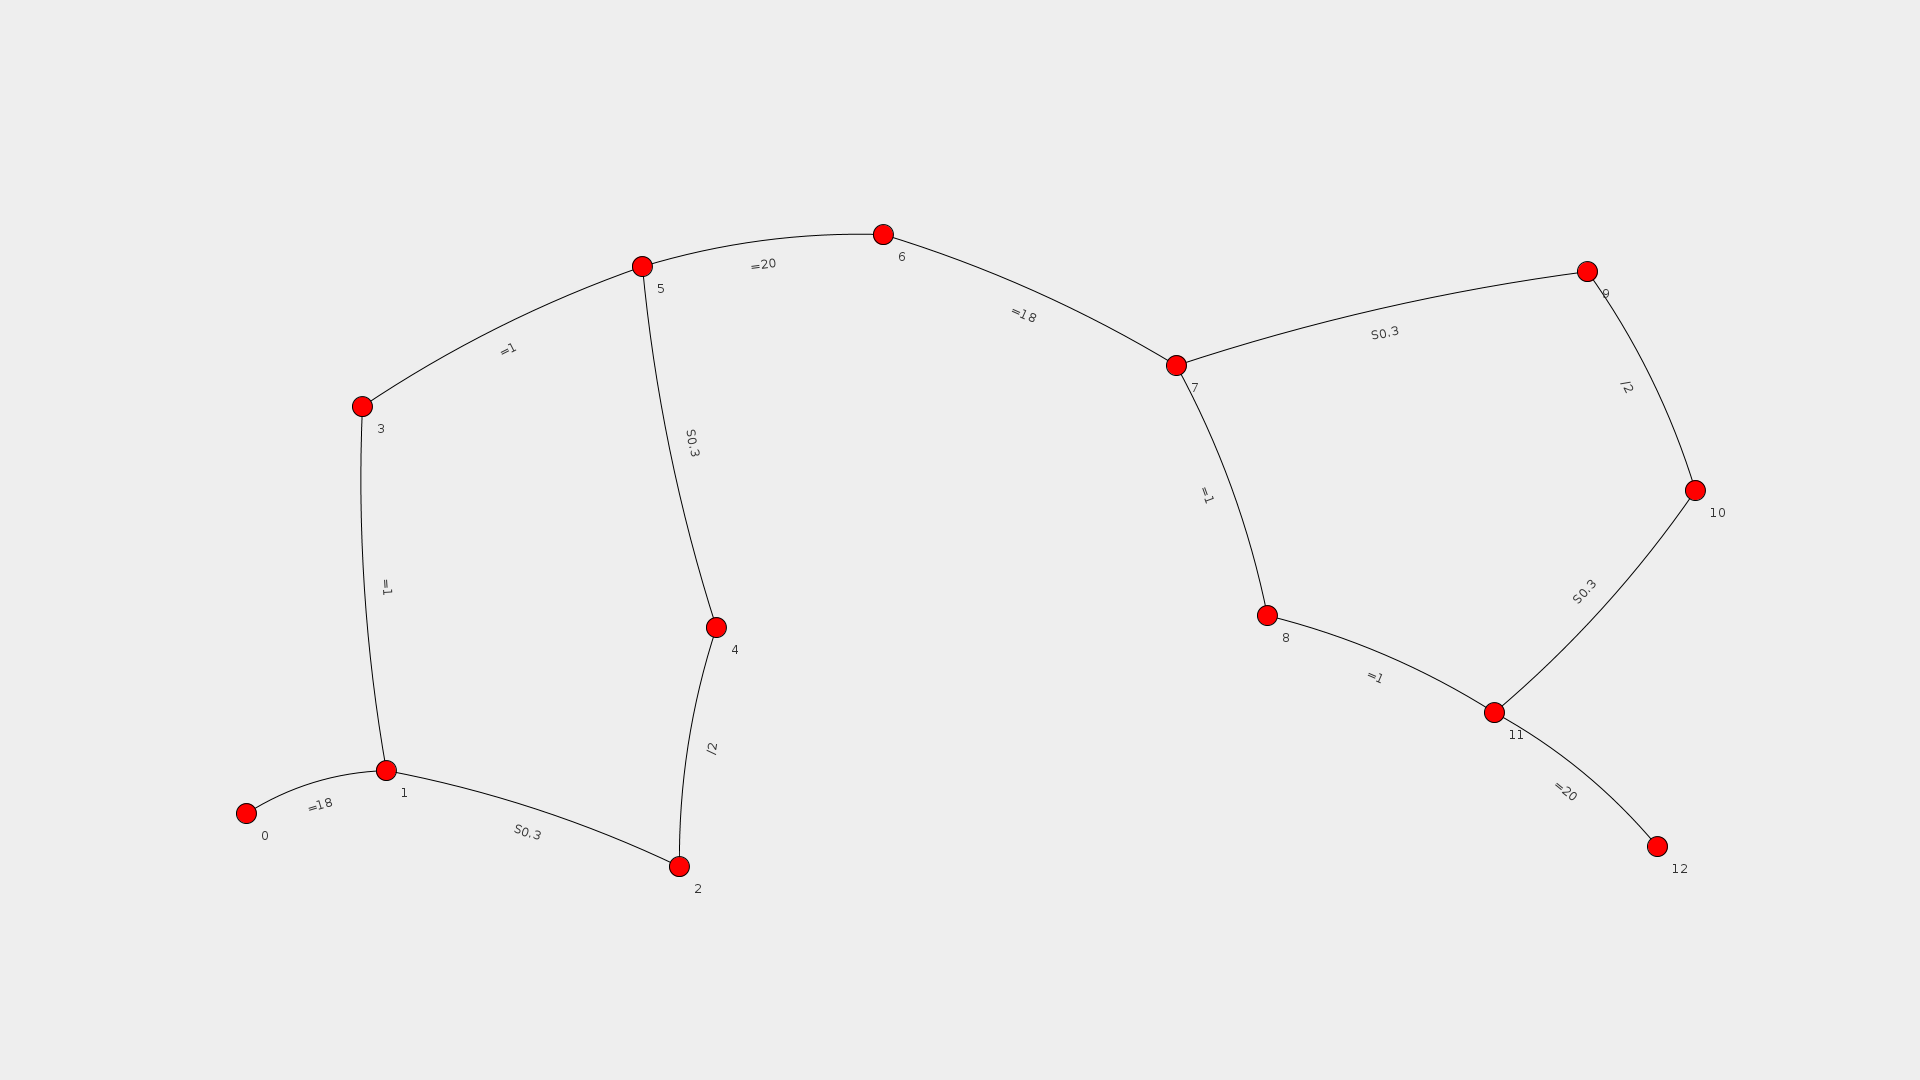
\includegraphics[width=150mm,angle=90]{solution.png}
\caption{RAS DATA SET TOY example territory. Undirected graph, arcs have descriptions.}
\end{figure}

\begin{figure}
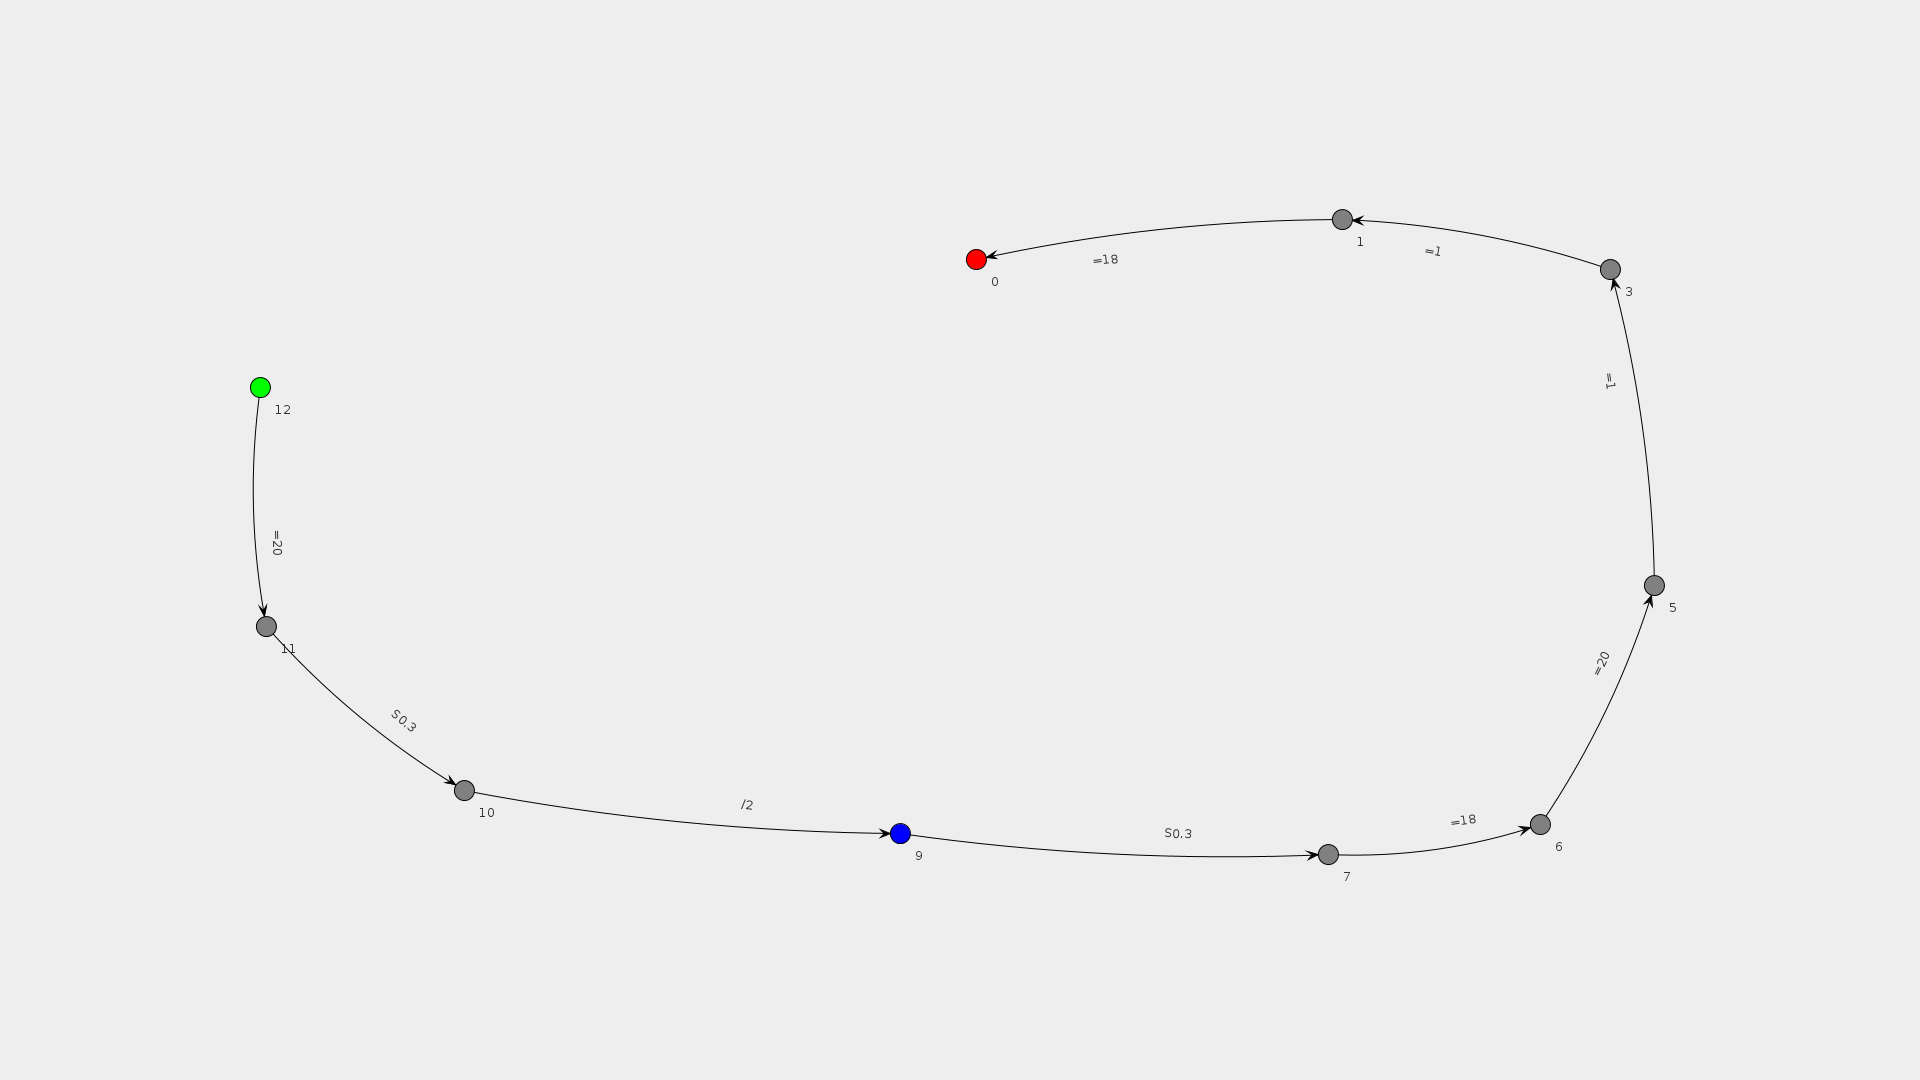
\includegraphics[width=150mm,angle=90]{B1.png}
\centering
\caption{RAS DATA SET TOY example, route of Train B1. Directed graph where green marks the origin, red the destination and blue is where the train is allowed to wait.}
\end{figure}

In this section, we show examples of visualizations that the solution is capable of providing. These visualizations have been rendered on the fly using the JUNG library\footnote{Java Universal Network/Graph framework, http://jung.sourceforge.net}.

\end{document}
